\documentclass[compress]{beamer} %en animé
%\documentclass[trans]{beamer} %en superposé

%%%%%%%%%%%%%% LES PACKAGES
\input{les_packages_pour_beamer.tex}
%%%%%%%%%%%%%% THEME BEAMER
%votre nom court qui apparaîtra dans l'en tête
\newcommand{\initiales}{Erwan FALAUX-BACHELOT}
\input{les_param_beamer_tipe}


%%%%%%%%%%%%%% MA PALETTE DE COULEURS
\input{la_palette.tex}
\definecolor{hellseahorse}{RGB}{204, 204, 255}
\definecolor{seahorse}{RGB}{204,180, 255}
\definecolor{darkseahorse}{RGB}{83, 74, 196}

%symboles pratiques
\newcommand{\flch}{\item[$\rightarrow$]}
\newcommand{\dc}{{\usebeamercolor[fg]{structure}$\hookrightarrow$}}
\newcommand{\ok}{\textcolor{vert}{\checkmark}}
\newcommand{\point}{{\usebeamercolor[fg]{structure}$\bullet\enskip$}}
\newcommand{\Point}{{\usebeamercolor[fg]{structure}$\bullet\enskip$}}


%styles
\newcommand{\couleur}[1]{{\usebeamercolor[fg]{structure}#1}}
\newcommand{\important}[1]{\couleur{\textbf{#1}}}
\newcommand{\remarque}[1]{\textit{\textrm{#1}}}

%pour le template
\newcommand{\lin}[1]{\mintinline{latex}{#1}}
%%%%%%%%%%%%%%%%%%%%%%%%%%%%%%%%%%%%%%%%%%%%%%%%%
\begin{document}
%

%%%%%%%%%%%%%%%%%%%%%%%%%%%%%%%%%%%%%%%%%%%%%%%%%
% A COMPLETER 
%%%%%%%%%%%%%%%%%%%%%%%%%%%%%%%%%%%%%%%%%%%%%%%%%

%entre crochet le titre court pour l'en tête puis le vrai titre
\title[La Transpilation]{
La transpilation de Fortran vers C
}

\author{
    \large 
    Présentation de \important{Erwan FALAUX-BACHELOT} (n° \important{33293})\\[0.2cm]
    \footnotesize
    travail réalisé avec \couleur{Yann MIQUEL--ERDMANN}\\[0.4cm]
    \vspace*{-1.2cm}
} 

%entre crochet la short date pour l'en-tête
\date[Juillet 2025]{}

\institute{}


%------------------------------------------------
\begin{frame}[plain]
    \titlepage 
    \addtocounter{framenumber}{-1}
\end{frame}

%------------------------------------------------
\title[Transpilation : conversion du Fortran vers le C]{
    Une page de titre avec logos :\\
    {\large mais sans les affectations détaillées des auteurs }
}


\begin{frame}
    \frametitle{Introduction\esp}

	\vspace{1.5cm}
    \begin{minipage}[t]{0.48\textwidth}
        \includegraphics[scale=0.05]{static/Fortran_logo.svg.png}\\
        \textbf{Le Fortran:}\\ 
        Créé par:  John Backus, IBM\\
        Créé en:   1957\\
        Dernière version en: 2023\\
        Rang sur Github: $41^{\text{ème}}$
    \end{minipage}
    \hspace*{0.2cm}
    \begin{minipage}[t]{0.48\textwidth}
        \includegraphics[scale=0.05]{static/C_logo.png}\\
        \textbf{Le C:}\\
        Créé par: Dennis Ritchie et \\Kenneth Thompson, Bell Labs\\
        Créé en:  1972\\
        Dernière version en: 2024\\
        Rang sur Github: $9^{\text{ème}}$
    \end{minipage}
    
	\vspace*{1.9cm}

    \bandeauREF{
        \hspace*{0.2cm}\textbf{Logo Fortran}: \url{https://commons.wikimedia.org/wiki/File:Fortran_logo.svg}\\
        \hspace*{0.2cm}\textbf{Logo C}: \url{https://commons.wikimedia.org/wiki/File:C_Logo.png}
    }

\end{frame}


\begin{frame}
    \frametitle{Problématique\esp}
    
    \begin{center}
        \textbf{Comment implémenter une conversion rapide de programmes Fortran en programmes C?}
    \end{center}

\end{frame}



\tikzstyle{lien} = [->, >=latex]
\tikzstyle{basic_text}=[text width=2cm, text badly centered]
\tikzstyle{basic_node}=[draw = black,rounded corners=4pt, basic_text]
\tikzstyle{wrapper}=[basic_node, inner sep=3pt]
\tikzstyle{hidden}=[draw=black!0,color=black!0]
\tikzstyle{faded}=[draw=black!20, color=black!20]

\section{La transpilation}

\begin{frame}
<<<<<<< Updated upstream
<<<<<<< Updated upstream
    \frametitle{Définition}
    \input{tikz/FortranVersC.tex}
=======
=======
>>>>>>> Stashed changes
    \frametitle{Définition\esp}
    schéma avec un fichier Fortran, une machine et un fichier fortran
    et 
    programme fortran en entrée hello world et le programme obtenu en sortie 
>>>>>>> Stashed changes
\end{frame}


\begin{frame}
<<<<<<< Updated upstream
<<<<<<< Updated upstream

    \frametitle{Les étapes de la transpilation}

   \begin{tikzpicture}
  %placer les éléments
  \node[draw, rounded corners] (1) at (0,0) {Analyse lexicale Fortran};
  \node[draw, rounded corners] (2) [right=1cm of 1] {Analyse syntaxique Fortran};
  \node[fit=(1)(2), fill=briqueRouge, opacity=0.5, inner sep=0.1em, rounded corners] {};

  \node[draw,fill=vertdEau, rounded corners] (3) [right=1cm of 2] {Traduction Vers C};
  \node[draw,fill=vertdEau, rounded corners] (4) [above right =1cm of 2 ] {Traduction Vers Python};
  \node[draw,fill=vertdEau, rounded corners] (5) [below right =1cm of 2 ] {Traduction Vers Fortran};


  %les relier
  \draw[black, line width = 1pt, ->, >=latex] (1) -- (2);
  \draw[black, line width = 1pt, ->, >=latex] (2) -- (3);
  \draw[black, line width = 1pt, ->, >=latex] (2) -- (4);
  \draw[black, line width = 1pt, ->, >=latex] (2) -- (5);
  
\end{tikzpicture}

=======
=======
>>>>>>> Stashed changes
    \frametitle{\esp}
    parties d'un transpileur
    schéma tikz explication des différents paramètres (langage d'entrée et celui de sortie et le fait que ces langages sont constants pour le transpileur ) 
>>>>>>> Stashed changes
\end{frame}



\begin{frame}
    \frametitle{Un peu plus de détails}
    \begin{tikzpicture}
  \node[basic_node] (A) at (0, 0) {Analyse lexicale};
  \node[basic_node] (B) [right=0.5cm of A] {Analyse syntaxique};
  \node[basic_node, minimum height=1cm] (C) [right=0.5cm of B] {Abstraction};
  \node[wrapper, fit=(A)(B)(C), draw=blue, hidden] (blue_fit) {};

  \node[basic_node] (D) [right = 0.75cm of C] {Conversion vers C};
  \node[basic_node, hidden] (E) [above = 0.75cm of D] {Conversion langage A};
  \node[basic_node, hidden] (F) [below = 0.75cm of D] {Conversion langage C};
  
  \node[wrapper, fit=(D), draw=red, hidden] (red_fit_1) {};
  \node[wrapper, fit=(E), draw=red, hidden] (red_fit_2) {};
  \node[wrapper, fit=(F), draw=red, hidden] (red_fit_3) {};

  \draw [lien] (A) -- (B);
  \draw [lien] (B) -- (C);
  \draw [lien] (C) -- (D);
  \draw [lien, hidden] (C) to [bend left] (E.west); 
  \draw [lien, hidden] (C) to [bend right] (F.west); 

  \node[fit=(red_fit_1)(red_fit_2)(red_fit_3)(blue_fit)] (global_fit) {};
  
  \node[below=2cm of global_fit.west, anchor=west, color=blue, hidden] (label1) {Module du langage d'entrée A};
  \node[below=0.5cm of label1.west, anchor=west, color=red, hidden] {Modules des langages de sortie};

\end{tikzpicture}
\end{frame}
\section{Analyse Lexicale}
%----------------regex----------------
\subsection{Les expressions régulières}
\tikzstyle{box}=[draw, rounded corners=4pt]
\tikzstyle{frame}=[box, minimum width=11.3cm, minimum height=6cm]
\tikzstyle{faded}=[color=black!25]
\tikzstyle{hidden}=[draw=white!0, color=white!0]

\begin{frame}
  \frametitle{Les expressions régulières}
  \begin{tikzpicture}
    % frame
    \node[frame] (frame) {};

    \node[below=0.5cm of frame.north west, anchor=north west] (1) {\point Expressions régulières};
    \node[faded, below=0.6cm of 1.west, anchor=west] {\point Automates};
    
    \node[below=4cm of frame.west, anchor=west, box] (state_1) {\scriptsize Analyse Lexicale};
    \node[right=0.5cm of state_1.east, anchor=west, box, faded] (state_2) {\scriptsize Analyse Syntaxique};
    \node[right=0.5cm of state_2.east, anchor=west, box, faded] (state_3) {\scriptsize Syntaxe Abstraite};
    \node[right=0.5cm of state_3.east, anchor=west, box, faded] (state_4) {\scriptsize Conversion};
    \draw[->, >=latex, faded] (state_1.east) -- (state_2.west);
    \draw[->, >=latex, faded] (state_2.east) -- (state_3.west);
    \draw[->, >=latex, faded] (state_3.east) -- (state_4.west);
    \draw[dashed] (frame.south west) -- (state_1.north west);
    \draw[dashed] (frame.south east) -- (state_1.north east);

    % definition
    \only<1->{
      \node[right=1.5 cm of 1] (def) {définies inductivement sur:};
      \node[below] at (def.south) (_1) {$\emptyset,\,\varepsilon,\, a \in\Sigma$};
    }
    \only<2->{
      \node[below=0.35cm] at (_1.south) (_2) {avec les règles usuelles:};
      \node[below] at (_2.south) (_3) {$\cdot,\ |,\ *$ };
    }
    \only<3->{
      \node[below=0.35cm] at (_3.south) (_4) {et des additionnelles:};
      \node[below] at (_4.south) {$+,\ ?,\ [a-z],\ \sim$};
    }

    % exemple
    \only<4->{
      \node[below=1.6cm of 1.south] (exmpl) {$\ \ $exemple:};
      \node[below, anchor=north east] (part1) at (exmpl.south) {[0 - 9]+}; \node[right=-3pt] (part2) at (part1.east) {(.[0 - 9]+)?};
    }
    \only<5->{\node[fit=(part1), draw=blue, rounded corners=4pt, inner sep=-1.5pt]{};}
    \only<6->{\node[fit=(part2), draw=red, rounded corners=4pt, inner sep=-1.5pt]{};}
  \end{tikzpicture}
\end{frame}

%---------------automates--------------
\subsection{Les automates}
\begin{frame}
  \frametitle{Les automates}
  \begin{tikzpicture}
    % frame
    \node[frame] (frame) {};

    \node[below=0.5cm of frame.north west, anchor=north west, faded] (1) {\point Expressions régulières};
    \node[below=0.6cm of 1.west, anchor=west] (_2) {\point Automates};

    \node[below=4cm of frame.west, anchor=west, box] (state_1) {\scriptsize Analyse Lexicale};
    \node[right=0.5cm of state_1.east, anchor=west, box, faded] (state_2) {\scriptsize Analyse Syntaxique};
    \node[right=0.5cm of state_2.east, anchor=west, box, faded] (state_3) {\scriptsize Syntaxe Abstraite};
    \node[right=0.5cm of state_3.east, anchor=west, box, faded] (state_4) {\scriptsize Conversion};
    \draw[->, >=latex, faded] (state_1.east) -- (state_2.west);
    \draw[->, >=latex, faded] (state_2.east) -- (state_3.west);
    \draw[->, >=latex, faded] (state_3.east) -- (state_4.west);
    \draw[dashed] (frame.south west) -- (state_1.north west);
    \draw[dashed] (frame.south east) -- (state_1.north east);

    % definition
    \only<1->{\node[right=4.5 cm of _2] (def) {$(\Sigma, Q, I, F, \delta)$};}
    \only<2->{
      \begin{scope}
        [below=1.5cm of def.south, scale=0.8, every node/.style={scale=0.8}, initial text=, shift={(0.8, 0)}]

        \node [state, initial]         (1) at (0, 0)        {1};
        \node [state]                  (2) [right=1cm of 1] {2};
        \node [state, accepting right] (3) [right=1cm of 2] {3};

        \path[->]
        (1) edge              node [above] {a} (2)
        (2) edge              node [above] {c} (3)
        (2) edge [loop above] node [above] {b} (2)
        ;
      \end{scope}
      \node [below=2.2cm of def.south, font=\scriptsize] {automate pour $a\cdot b*\cdot c$};
    }
  \end{tikzpicture}
\end{frame}

%------------étude d'un exemple-----------
\begin{frame}
  \frametitle{Les automates: étude d'un exemple}
  \begin{tikzpicture}
    \begin{scope}
      [every node/.style={scale=0.6,font=\Large}, scale=0.4, initial text=]
      \tikzstyle{style0}=[draw=black]
      \tikzstyle{style1}=[draw=black]
      \tikzstyle{style2}=[draw=black]
      \tikzstyle{style3}=[draw=black]
      \tikzstyle{style4}=[draw=black]
      \tikzstyle{style5}=[draw=black]
      \tikzstyle{style6}=[draw=black]
      \tikzstyle{style7}=[draw=black]
      \tikzstyle{style8}=[draw=black]
      \tikzstyle{style9}=[draw=black]

      \only<1> {\tikzstyle{style0}=[draw=blue!50,very thick,fill=blue!20]}
      \only<2> {\tikzstyle{style1}=[draw=blue!50,very thick,fill=blue!20]}
      \only<3> {\tikzstyle{style2}=[draw=blue!50,very thick,fill=blue!20]}
      \only<4> {\tikzstyle{style3}=[draw=blue!50,very thick,fill=blue!20]}
      \only<5> {\tikzstyle{style4}=[draw=blue!50,very thick,fill=blue!20]}
      \only<6> {\tikzstyle{style5}=[draw=blue!50,very thick,fill=blue!20]}
      \only<7> {\tikzstyle{style0}=[draw=blue!50,very thick,fill=blue!20]}
      \only<8> {\tikzstyle{style8}=[draw=blue!50,very thick,fill=blue!20]}
      \only<9> {\tikzstyle{style0}=[draw=blue!50,very thick,fill=blue!20]}
      \only<10>{\tikzstyle{style9}=[draw=blue!50,very thick,fill=blue!20]}
      \only<11> {\tikzstyle{style0}=[draw=blue!50,very thick,fill=blue!20]}
      \only<12-23>{\tikzstyle{style6}=[draw=blue!50,very thick,fill=blue!20]}
      \only<24>{\tikzstyle{style7}=[draw=blue!50,very thick,fill=blue!20]}

      \node[state, style0, initial        ]  at (0,0) (0)          {$I$};

      \node[state, style1] (1) at (2,1) {1};
      \node[state, style2] (2) [right=0.4cm of 1] {2};
      \node[state, style3] (3) [right=0.4cm of 2] {3};
      \node[state, style4] (4) [right=0.4cm of 3] {4};
      \node[state, accepting right, style5] (5) [right=0.4cm of 4] {$F_1$};
      
      \node[state, style6,                ] (6) at (2,3) {5};
      \node[state, style7, accepting right] (7) [right=0.4cm of 6] {$F_2$};
      
      \node[state, style8, accepting right] (8) at (2,-1)      {$F_3$};
      \node[state, style9, accepting right] (9) at (2,-3)      {$F_4$};

      \path[->]
      (0) edge                node[above] {$*$} (8)
      (0) edge                node[above] {\LARGE$,$} (9)

      (0) edge                node[above] {$p$} (1)
      (1) edge                node[above] {$r$} (2)
      (2) edge                node[above] {$i$} (3)
      (3) edge                node[above] {$n$} (4)
      (4) edge                node[above] {$t$} (5)
      
      
      (0) edge                node[above] {$"$} (6)
      (6) edge [loop above]   node[above] {\large$[a-zA-Z0-9\_]$} (6)
      (6) edge                node[above] {$"$} (7)
      ;
      
    \end{scope}
    \node at (8, 0) (text) {\ttfamily print*,"Hello World"};
    \foreach \step in {1,2,...,6}{
      \node<\step>[right=\fpeval{\step * 5.75 - 3}pt of text.west, draw=blue, fill=blue!20, inner sep=0pt, minimum width=2pt, minimum height=10pt]{};
    }
    \foreach \step in {7,8}{
      \node<\step>[right=\fpeval{(\step - 1) * 5.75 - 3}pt of text.west, draw=blue, fill=blue!20, inner sep=0pt, minimum width=2pt, minimum height=10pt]{};
    }
    \foreach \step in {9,10}{
      \node<\step>[right=\fpeval{(\step - 2) * 5.75 - 3}pt of text.west, draw=blue, fill=blue!20, inner sep=0pt, minimum width=2pt, minimum height=10pt]{};
    }
    \foreach \step in {11,12,...,24}{
      \node<\step>[right=\fpeval{(\step - 3) * 5.75 - 3}pt of text.west, draw=blue, fill=blue!20, inner sep=0pt, minimum width=2pt, minimum height=10pt]{};
    }
    \node at (1, -2.3) (lb) {\texttt{res = [}};
    \only<7-> {\node [right] at (lb.east) (lb) {\texttt{'print'}};}
    \only<9-> {\node [right] at (lb.east) (lb) {\texttt{, '*'}};} 
    \only<11-> {\node [right] at (lb.east) (lb) {\texttt{, ','}};}
    \only<25> {\node [right] at (lb.east) (lb) {\texttt{, '"Hello World"'}};}
    \node [right] at (lb.east) {\texttt{]}};
  \end{tikzpicture}
\end{frame}

%------------déterminisation-----------
\addtocounter{framenumber}{-1}
\subsection{La déterminisation}
\begin{frame}
  \addtocounter{framenumber}{1}
  \frametitle{La déterminisation}

  \begin{tikzpicture}
    % frame
    \begin{scope}
      \node[frame] (frame) {};
      
      \node[below=4cm of frame.west, anchor=west, box] (state_1) {\scriptsize Analyse Lexicale};
      \node[right=0.5cm of state_1.east, anchor=west, box, faded] (state_2) {\scriptsize Analyse Syntaxique};
      \node[right=0.5cm of state_2.east, anchor=west, box, faded] (state_3) {\scriptsize Syntaxe Abstraite};
      \node[right=0.5cm of state_3.east, anchor=west, box, faded] (state_4) {\scriptsize Conversion};
      \draw[->, >=latex, faded] (state_1.east) -- (state_2.west);
      \draw[->, >=latex, faded] (state_2.east) -- (state_3.west);
      \draw[->, >=latex, faded] (state_3.east) -- (state_4.west);
      \draw[dashed] (frame.south west) -- (state_1.north west);
      \draw[dashed] (frame.south east) -- (state_1.north east);
    \end{scope}

    % automatons
    \only<1,2>{
      \begin{scope}[initial text=, scale=0.9, shift={(-5, 0)}]
        \node[state, initial] (0) at (0, 0) {0};
        \node[state] (1) at (1.3, 1) {1};
        \node[state] (2) at (1.3, -1) {2};
        \node[state, right=0.5cm of 1, accepting right] (3) {3};
        \node[state, right=0.5cm of 2, accepting right] (4) {4};

        \path[->]
        (0) edge node[above] {a} (1)
        (0) edge node[above] {a} (2)
        (1) edge node[above] {b} (3)
        (2) edge node[above] {c} (4)
        ;
      
      \end{scope}
    }
      
    \only<1,3>{
      \begin{scope}[shift={(1.4, 0)}, initial text=, scale=0.9]
        \node[state, initial] (0) at (0, 0) {0};
        \node[state, right=0.5cm of 0] (1) {\{1,2\}};
        \node[state, accepting right] (3) at (3.3, 1) {3};
        \node[state, accepting right] (4) at (3.3, -1) {4};

        \path[->]
        (0) edge node[above] {a} (1)
        (1) edge node[above] {b} (3)
        (1) edge node[above] {c} (4)
        ;
      \end{scope}
    }

    \only<2>{
      \begin{scope}[shift={(2.5, 0)}]
        \node{
          \begin{minipage}{0.55\textwidth}
            \inputminted[firstline=7, lastline=12,firstnumber=1]{ocaml}{scripts/automates.ml}
          \end{minipage}
        };
      \end{scope}
    }

    \only<3>{
      \begin{scope}[shift={(-2.5, 0)}]
        \node{
          \begin{minipage}{0.55\textwidth}
            \inputminted[firstline=29, lastline=34,firstnumber=1]{ocaml}{scripts/automates.ml}
          \end{minipage}
        };
      \end{scope}
    }
  \end{tikzpicture}
\end{frame}

\section{Analyse Syntaxique}

\tikzstyle{box}=[draw, rounded corners=4pt]
\tikzstyle{frame}=[box, minimum width=11.3cm, minimum height=6cm]
\tikzstyle{faded}=[color=black!25]
\tikzstyle{hidden}=[draw=white!0, color=white!0]

%------------grammaire-----------
\subsection{La grammaire}
\begin{frame}
  \frametitle{Analyse Syntaxique}

  \begin{tikzpicture}
    % frame
    \node[frame] (frame) {};

    \node[below=0.5cm of frame.north west, anchor=north west] (1) {\point Grammaire};
    \node[faded, below=0.6cm of 1.west, anchor=west] (_2) {\point LL1};

    \tikzstyle{faded}=[draw=black!20,color=black!20]
    \node[below=4cm of frame.west, anchor=west, box, faded] (state_1) {\scriptsize Analyse Lexicale};
    \node[right=0.5cm of state_1.east, anchor=west, box] (state_2) {\scriptsize Analyse Syntaxique};
    \node[right=0.5cm of state_2.east, anchor=west, box, faded] (state_3) {\scriptsize Syntaxe Abstraite};
    \node[right=0.5cm of state_3.east, anchor=west, box, faded] (state_4) {\scriptsize Conversion};
    \draw[->, >=latex, faded] (state_1.east) -- (state_2.west);
    \draw[->, >=latex, faded] (state_2.east) -- (state_3.west);
    \draw[->, >=latex, faded] (state_3.east) -- (state_4.west);
    \draw[dashed] (frame.south west) -- (state_2.north west);
    \draw[dashed] (frame.south east) -- (state_2.north east);

    % définition
    \only<1->{
      \node[right=3.2cm of 1.east, anchor=west] (def) {Règles de production:};
      \node[below=0.25cm, font=\ttfamily] (def1) at (def) {A -> B};
      \node[below=0.25cm, font=\ttfamily] (def2) at (def1) {A -> $c, c\in \Sigma^*$};
    }

    % exemple simple
    \only<2->{
      \node[below=0.5cm of def2]{Exemple:};
      \node[below=2.3cm of def.200, anchor = north west] {
        \begin{minipage}{0.5\textwidth}
          \inputminted{text}{static/Grammaire_example.txt}
        \end{minipage}
      };
    }

    % application à une chaine simple
    \only<3->{
      \begin{scope}[scale=1, shift={(-2, 1.8)}, font=\footnotesize]
      
        \node (0) at (0, 0) {S};
        \node [below=0.3cm of 0] (1) {A};
        \node [below=0.3cm of 1.south west] (2) {a};
        \node [below=0.3cm of 1.south east] (3) {A};
        \node [below=0.3cm of 3] (4) {B};
        \node [below=0.3cm of 4.south west] (5) {b};
        \node [below=0.3cm of 4.south east] (6) {B};
        \node [below=0.3cm of 6] (7) {$\varepsilon$};

        \node [below=0.1cm of 7] {Arbre de dérivation de ab};

        \draw (0) -- (1);
        \draw (1) -- (2);
        \draw (1) -- (3);
        \draw (3) -- (4);
        \draw (4) -- (5);
        \draw (4) -- (6);
        \draw (6) -- (7);
      \end{scope}
    }

  \end{tikzpicture}

\end{frame}

%-------------LL1--------------
\subsection{L'algorithme LL1}
\begin{frame}
  \begin{tikzpicture}
    % frame
    \node[frame] (frame) {};

    \node[below=0.5cm of frame.north west, anchor=north west, faded] (1) {\point Grammaire};
    \node[below=0.6cm of 1.west, anchor=west] (_2) {\point LL1};

    \tikzstyle{faded}=[draw=black!20,color=black!20]
    \node[below=4cm of frame.west, anchor=west, box, faded] (state_1) {\scriptsize Analyse Lexicale};
    \node[right=0.5cm of state_1.east, anchor=west, box] (state_2) {\scriptsize Analyse Syntaxique};
    \node[right=0.5cm of state_2.east, anchor=west, box, faded] (state_3) {\scriptsize Syntaxe Abstraite};
    \node[right=0.5cm of state_3.east, anchor=west, box, faded] (state_4) {\scriptsize Conversion};
    \draw[->, >=latex, faded] (state_1.east) -- (state_2.west);
    \draw[->, >=latex, faded] (state_2.east) -- (state_3.west);
    \draw[->, >=latex, faded] (state_3.east) -- (state_4.west);
    \draw[dashed] (frame.south west) -- (state_2.north west);
    \draw[dashed] (frame.south east) -- (state_2.north east);

    % petite description de LL1
    \node[font=\ttfamily] (list) at (-4, 0){[a, b]};
    \node[right] (+) at (list.east) {$+$};
    \node[right] at (+.east) {
        \begin{minipage}{0.5\textwidth}
          \inputminted{text}{static/Grammaire_example.txt}
        \end{minipage}
    };
    \only<1>{
      \node[font=\ttfamily] at (0.5, 0) {=>};
      \begin{scope}[shift={(2.5, 1.8)}, font=\footnotesize]
        
        \node (0) at (0, 0) {S};
        \node [below=0.3cm of 0] (1) {A};
        \node [below=0.3cm of 1.south west] (2) {a};
        \node [below=0.3cm of 1.south east] (3) {A};
        \node [below=0.3cm of 3] (4) {B};
        \node [below=0.3cm of 4.south west] (5) {b};
        \node [below=0.3cm of 4.south east] (6) {B};
        \node [below=0.3cm of 6] (7) {$\varepsilon$};

        \draw (0) -- (1);
        \draw (1) -- (2);
        \draw (1) -- (3);
        \draw (3) -- (4);
        \draw (4) -- (5);
        \draw (4) -- (6);
        \draw (6) -- (7);
      \end{scope}
    }
    
  \end{tikzpicture}

\end{frame}
\section{Conversion vers la syntaxe abstraite}

% TODO ajouter ici une diapo pour expliquer le but général (arbre donné trop gros + pas adapté pour les autres langages que fortran, on le transforme en un arbre de syntaxe abstraite)

\begin{frame}
  \frametitle{Principe général de l'abstraction}
  \begin{tikzpicture}
    \node (0, 0) {}; % to align the scope
    \begin{scope} [shift={(5.5, 0)}]
      \node [basic_node, text width=7cm, align=left] (Fortran) {
        \scalebox{0.8}{\textbf{Arbre de syntaxe}} 
        \scalebox{0.6}{    
\tikzstyle{feuille}=[ draw, rectangle, inner sep = 0.12cm]
\tikzstyle{noeud}=[ draw, rectangle,rounded corners, minimum width= 0.64cm, line width = 1pt]
\begin{tikzpicture}[
        baseline=(base), 
        level/.style={sibling distance = 1.6cm/#1, level distance = 1cm},
        every node/.style={scale=0.6, font=\footnotesize}
    ]
    
    \node[ noeud] {Programme}
    child { 
        node[noeud] (base) {ProgramMC}
    }
    child {
        node[noeud] {NomProg}
        child {node[feuille] {"hello"}}
    }
    child [ level distance=2cm]{ 
        node [ noeud] {Print}
        child [sibling distance= 1cm] {
            node [noeud] {PrintMC}
        }
        child [sibling distance= 1cm]{
            node [noeud] {Asterisque}
        }
        child [sibling distance= 1cm]{
            node [noeud] {Virgule}
        }
        child [sibling distance= 1cm]{
            node [noeud] {Chaine}
            child { 
                node [feuille] {"Hello World"}
            }
        }
        child [sibling distance= 1cm] {
            node [noeud] {Paramliste}
            child { 
                node [feuille] {$\varepsilon$}
            }
        }
    }
    child { 
        node[ noeud] {EndProgramMC}
    }
    child {
        node[noeud] {NomProg}
        child {node[feuille] {"hello"}}
    };

\end{tikzpicture}}
      };

      \node [basic_node, text width=5.5cm, below=1cm of Fortran, align=left] (C) {
        \scalebox{0.8}{\textbf{Arbre de syntaxe abstraite}}
        \scalebox{0.9}{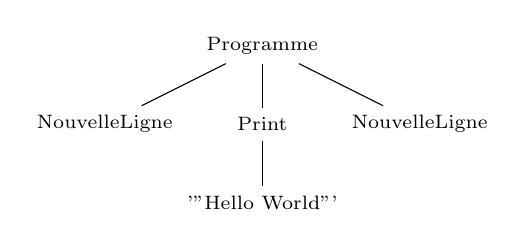
\begin{tikzpicture}
    \node[font=\scriptsize] (0) at (0, 0) {Programme};
    \node[font=\scriptsize] (1) at (-2, -1) {NouvelleLigne};
    \node[font=\scriptsize] (2) at (0, -1) {Print};
    \node[font=\scriptsize] (3) at (0, -2) {'"Hello World"'};
    \node[font=\scriptsize] (4) at (2, -1) {NouvelleLigne};
    
    \draw (0) -- (1);
    \draw (0) -- (2);
    \draw (2) -- (3);
    \draw (0) -- (4);
\end{tikzpicture}}
      };

      \draw [lien, thick] (Fortran.south) to (C.north);
    \end{scope}
  \end{tikzpicture}
\end{frame}

\newcommand{\drawcross}[1]{
  \draw[cross] (#1.north west) -- (#1.south east);
  \draw[cross] (#1.north east) -- (#1.south west);
}

\tikzstyle{cross}=[red, very thick]

%--------------expilaction---------------
\subsection{Fonctionnement}
\begin{frame}
  \frametitle{Syntaxe abstraite\esp}

  \begin{tikzpicture}
    % frame
    \node[frame] (frame) {};
    \tikzstyle{faded}=[draw=black!20,color=black!20]
    
    \node[below=4cm of frame.west, anchor=west, box, faded] (state_1) {\scriptsize Analyse lexicale};
    \node[right=0.5cm of state_1.east, anchor=west, box, faded] (state_2) {\scriptsize Analyse syntaxique};
    \node[right=0.5cm of state_2.east, anchor=west, box] (state_3) {\scriptsize Abstraction};
    \node[right=0.5cm of state_3.east, anchor=west, box, faded] (state_4) {\scriptsize Conversion};
    \draw[->, >=latex, faded] (state_1.east) -- (state_2.west);
    \draw[->, >=latex, faded] (state_2.east) -- (state_3.west);
    \draw[->, >=latex, faded] (state_3.east) -- (state_4.west);
    \draw[dashed] (frame.south west) -- (state_3.north west);
    \draw[dashed] (frame.south east) -- (state_3.north east);

    % definition
    \begin{scope}[shift={(-3, 2)}, font=\footnotesize]
      \node (0) at (0, 0) {S};
      \node [below=0.3cm of 0] (1) {A};
      \node [below=0.3cm of 1.south west] (2) {a};
      \node [below=0.3cm of 1.south east] (3) {A};
      \node [below=0.3cm of 3] (4) {B};
      \node [below=0.3cm of 4.south west] (5) {b};
      \node [below=0.3cm of 4.south east] (6) {B};
      \node [below=0.3cm of 6] (7) {$\varepsilon$};

      \draw (0) -- (1);
      \draw (1) -- (2);
      \draw (1) -- (3);
      \draw (3) -- (4);
      \draw (4) -- (5);
      \draw (4) -- (6);
      \draw (6) -- (7);
    
      
      \only<2->{\drawcross{3}}
      \only<3->{\drawcross{6}}
      \only<4->{\drawcross{7}}
      
      \only<5->{
        \node[right=0.8cm of 3, font=\ttfamily] {$\Rightarrow$};

        \node [right=2.5cm of 0] (_0) {S};
        \node [below=0.3cm of _0] (_1) {A};
        \node [below=0.3cm of _1.south west] (_2) {a};
        \node [below=0.3cm of _1.south east] (_4) {B};
        \node [below=0.3cm of _4.south] (_5) {b};

        \draw (_0) -- (_1);
        \draw (_1) -- (_2);
        \draw (_1) -- (_4);
        \draw (_4) -- (_5);
      }

      \only<6->{\draw[->, >=latex, draw=blue, very thick] (_4) [bend right] to (_0);}

      \only<7>{
        \node[right=0.8cm of _4, font=\ttfamily] {$\Rightarrow$};

        \node [right=2.5cm of _1] (__0) {S};
        \node [below=0.3cm of __0.south west] (__1) {A};
        \node [below=0.3cm of __1.south] (__2) {a};
        \node [below=0.3cm of __0.south east] (__4) {B};
        \node [below=0.3cm of __4.south] (__5) {b};

        \draw (__0) -- (__1);
        \draw (__1) -- (__2);
        \draw (__0) -- (__4);
        \draw (__4) -- (__5);
        }
    \end{scope}

  \end{tikzpicture}

\end{frame}

%----------un exemple----------
\subsection{Un exemple}
\begin{frame}
  \scalebox{0.8}{\tikzstyle{feuille}=[]
\tikzstyle{noeud}=[]
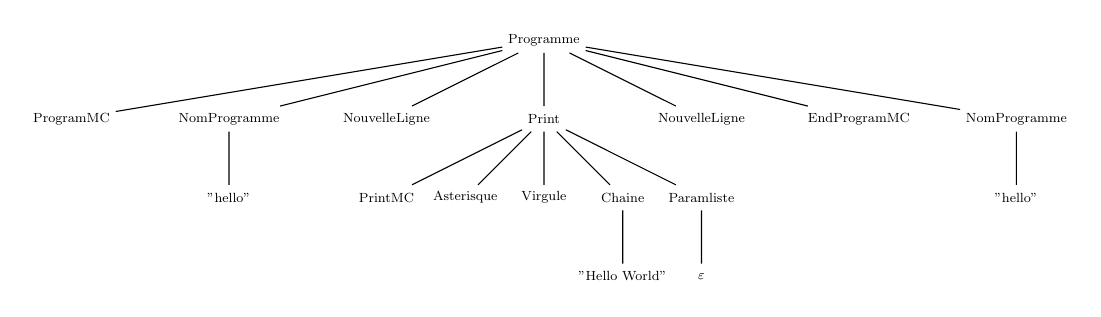
\begin{tikzpicture}
    [
        baseline=(0), 
        level/.style={sibling distance = 2cm/#1, level distance = 1cm},
        every node/.style={scale=0.6, font=\footnotesize, minimum width=15pt, minimum height=15pt}
    ]
    
    \node at (0, 0) { };
    \begin{scope}[shift={(5, 0)}]
        \node {Programme}
            child {node (0) {ProgramMC}}
            child {node (1) {NomProgramme}
                child {node (2) {"hello"}}
            }
            child {node {NouvelleLigne}}
            child {node {Print}
                child {node (3) {PrintMC}}
                child {node (4) {Asterisque}}
                child {node (5) {Virgule}}
                child {node (6) {Chaine}
                    child {node {"Hello World"}}
                }
                child{node (7) {Paramliste}
                    child {node (8) {$\varepsilon$}}
                }
            }
            child {node {NouvelleLigne}}
            child {node (9) {EndProgramMC}}
            child {node (10) {NomProgramme}
                child {node (11) {"hello"}}
            }
        ;
        \only<2>{\foreach \step in {0,1,...,11}{\drawcross{\step}}}
    \end{scope}
\end{tikzpicture}}
\end{frame}

\begin{frame}
  \begin{center}
    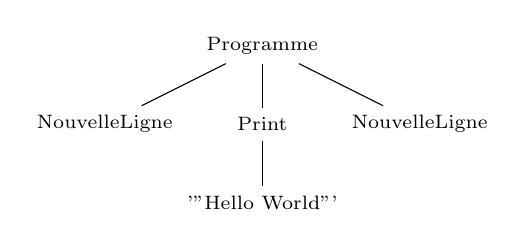
\begin{tikzpicture}
    \node[font=\scriptsize] (0) at (0, 0) {Programme};
    \node[font=\scriptsize] (1) at (-2, -1) {NouvelleLigne};
    \node[font=\scriptsize] (2) at (0, -1) {Print};
    \node[font=\scriptsize] (3) at (0, -2) {'"Hello World"'};
    \node[font=\scriptsize] (4) at (2, -1) {NouvelleLigne};
    
    \draw (0) -- (1);
    \draw (0) -- (2);
    \draw (2) -- (3);
    \draw (0) -- (4);
\end{tikzpicture}
  \end{center}
\end{frame}
\section{Traduction vers le langage de sortie}

% TODO ajouter une diapo pour expliquer le but général (transformer l'arbre de syntaxe abstraite vers le langage de sortie)

\begin{frame}
  \frametitle{Principe général de la traduction}
  \begin{tikzpicture}
    \node (0, 0) {}; % to align the scope
    \begin{scope} [shift={(5.5, 0)}]
      \node [basic_node, text width=5.5cm, align=left] (Fortran) {
        \scalebox{0.8}{\textbf{Arbre de syntaxe abstraite}}
        \scalebox{0.9}{\begin{tikzpicture}
    \node[font=\scriptsize] (0) at (0, 0) {Programme};
    \node[font=\scriptsize] (1) at (-2, -1) {NouvelleLigne};
    \node[font=\scriptsize] (2) at (0, -1) {Print};
    \node[font=\scriptsize] (3) at (0, -2) {'"Hello World"'};
    \node[font=\scriptsize] (4) at (2, -1) {NouvelleLigne};
    
    \draw (0) -- (1);
    \draw (0) -- (2);
    \draw (2) -- (3);
    \draw (0) -- (4);
\end{tikzpicture}}
      };

      \node [basic_node, text width=5.5cm, align=left, below=1cm of Fortran] (C) {
        \scalebox{0.8}{
          \parbox{\textwidth}{
            \textbf{Programme C}
            \inputminted{c}{static/HelloWorld.c}
          }
        } 
      };

      \draw [lien, thick] (Fortran.south) to (C.north);
    \end{scope}
  \end{tikzpicture}
\end{frame}

\begin{frame}
  \frametitle{Traduction\esp}

  \begin{tikzpicture}
    % frame
    \node[frame] (frame) {};
    \tikzstyle{faded}=[draw=black!20,color=black!20]
    
    \node[below=4cm of frame.west, anchor=west, box, faded] (state_1) {\scriptsize Analyse lexicale};
    \node[right=0.5cm of state_1.east, anchor=west, box, faded] (state_2) {\scriptsize Analyse syntaxique};
    \node[right=0.5cm of state_2.east, anchor=west, box, faded] (state_3) {\scriptsize Abstraction};
    \node[right=0.5cm of state_3.east, anchor=west, box] (state_4) {\scriptsize Conversion};
    \draw[->, >=latex, faded] (state_1.east) -- (state_2.west);
    \draw[->, >=latex, faded] (state_2.east) -- (state_3.west);
    \draw[->, >=latex, faded] (state_3.east) -- (state_4.west);
    \draw[dashed] (frame.south west) -- (state_4.north west);
    \draw[dashed] (frame.south east) -- (state_4.north east);

    \node(def) at (0, 0.5) {parcours en profondeur de l'AST};
    \node[below] at (def.south) {conversion en chaîne};

  \end{tikzpicture}

\end{frame}

\begin{frame}
    \usetikzlibrary {fit}
    \frametitle{Transpileur\esp}
    \begin{tikzpicture}
  \tikzstyle{blue_b}=[draw=white]
  \tikzstyle{blue_t}=[color=white]
  \tikzstyle{red_b}=[draw=white]
  \tikzstyle{red_t}=[color=white]
  \tikzstyle{out_b}=[draw=white]
  \tikzstyle{out_t}=[color=white]

  \only<2-4>{
    \tikzstyle{blue_b}=[draw=blue]
    \tikzstyle{blue_t}=[color=blue]
  }
  \only<3->{
    \tikzstyle{red_b}=[draw=red]
    \tikzstyle{red_t}=[color=red]
  }
  \only<4->{
    \tikzstyle{out_b}=[]
    \tikzstyle{out_t}=[]
  }
  \only<5>{
    \tikzstyle{blue_b}=[draw=vertFonce]
    \tikzstyle{blue_t}=[color=vertFonce]
  }

  \node[basic_node] (A) at (0, 0) {Analyse lexicale};
  \node[basic_node] (B) [right=0.5cm of A] {Analyse syntaxique};
  \node[basic_node, minimum height=1cm] (C) [right=0.5cm of B] {Abstraction};
  \node[wrapper, fit=(A)(B)(C), blue_b] (blue_fit) {};

  \node[basic_node] (D) [right = 0.75cm of C] {Conversion vers C};
  \node[basic_node, out_b, out_t] (E) [above = 0.75cm of D] {Conversion vers Fortran};
  \node[basic_node, out_b, out_t] (F) [below = 0.75cm of D] {Conversion vers Python};
  
  \node[wrapper, fit=(D), red_b] (red_fit_1) {};
  \node[wrapper, fit=(E), red_b, out_b] (red_fit_2) {};
  \node[wrapper, fit=(F), red_b, out_b] (red_fit_3) {};

  \draw [lien] (A) -- (B);
  \draw [lien] (B) -- (C);
  \draw [lien] (C) -- (D);
  \draw [lien, out_b] (C) to [bend left] (E.west); 
  \draw [lien, out_b] (C) to [bend right] (F.west); 

  \node[fit=(red_fit_1)(red_fit_2)(red_fit_3)(blue_fit)] (global_fit) {};
  
  \node[below=2cm of global_fit.west, anchor=west, blue_t] (label1) {Module du \only<1-4>{Fortran}\only<5>{C}};
  \node[below=0.5cm of label1.west, anchor=west, red_t] {Module\only<4->{s des langages de sortie}\only<1-3>{ du C}};

\end{tikzpicture}
\end{frame}

\begin{frame}
\noindent
\begin{minipage}[t]{0.47\textwidth}
    \scalebox{0.4}{
        \parbox{\textwidth}{
            \inputminted{fortran}{static/fibonacci.f90}
        }
    }
    
\end{minipage}
\hfill
\begin{minipage}[t]{0.52\textwidth}
    \scalebox{0.4}{
        \color{black!20}
        \vrule{\color{white}a}
        \color{black}
        \parbox{\textwidth}{
            \inputminted{c}{static/fibonacci.c}
        }
    }
\end{minipage}

\end{frame}

\begin{frame}
    \frametitle{Conclusion\esp}

    \point Conversion rapide: 10000 transpilations du fibonacci en 21s\\
    \point Partie automatisée rend la création moins pénible\\
    \point Processus interchangeable avec les langages souhaités

\end{frame}

%
\section{Annexe}

\foreach \name in{src/preprocessing/generateGrammar.ml, src/preprocessing/generateMlFiles.ml, src/prebuild/buildAutomaton.ml, src/abstractTokens.ml, src/bibliotheques.ml, src/environnement.ml, src/symbols.ml, src/traduction.ml, src/regex.ml, src/grammarFunctions.ml, src/grammar.ml, src/automates.ml, src/LL1.ml, src/convertToAbstract.ml, src/detAutomaton.ml, src/traductionC.ml, src/traductionFortran.ml, src/transpileurs.ml, src/main.ml}{
    \subsection{\name}
    \tiny   \inputminted[]{ocaml}{../../\name}
    
    \pagebreak
}


\end{document}